\section{GNSS}
    \begin{frame}{Coordenadas Geográficas}
        \begin{columns}
            \begin{column}{0.55\textwidth}
                \centering
                % \begin{tikzpicture}[scale=1,tdplot_main_coords,every node/.style={font = {\footnotesize\bfseries}}]
% https://latex.org/forum/viewtopic.php?t=25316

\def\rvec{3.5}

\def\phivecA{30}
\def\thetavecA{75}

\def\phivecB{45}
\def\thetavecB{15}

\def\auxOpacity{0.75}

\pgfmathsetmacro{\ax}{\rvec*sin(\phivecA)*cos(\thetavecA)}
\pgfmathsetmacro{\ay}{\rvec*sin(\phivecA)*sin(\thetavecA)}
\pgfmathsetmacro{\az}{\rvec*cos(\phivecA)}

\pgfmathsetmacro{\bx}{\rvec*sin(\phivecB)*cos(\thetavecB)}
\pgfmathsetmacro{\by}{\rvec*sin(\phivecB)*sin(\thetavecB)}
\pgfmathsetmacro{\bz}{\rvec*cos(\phivecB)}


\shadedraw[tdplot_screen_coords, ball color = white, opacity=0.25] (0,0) circle (\rvec);

%-----------------------
\coordinate (O) at (0,0,0);

\tdplotsetcoord{A}{\rvec}{\phivecA}{\thetavecA}

\tdplotsetcoord{B}{\rvec}{\phivecB}{\thetavecB}

\tdplotsetcoord{N}{\rvec}{0}{90}

%draw the main coordinate system axes
\draw[thick,-latex] (O) -- (1.35*\rvec,0,0) node[anchor=north east]{$x$};
\draw[thick,-latex] (O) -- (0,1.35*\rvec,0) node[anchor=north west]{$y$};
\draw[thick,-latex] (O) -- (0,0,1.35*\rvec) node[anchor=south]{$z$};

\draw[thick,-latex,opacity=0] (O) -- (-1.35*\rvec,0,0) node[anchor=south west]{$x$};
\draw[thick,-latex,opacity=0] (O) -- (0,-1.35*\rvec,0) node[anchor=south east]{$y$};
\draw[thick,-latex,opacity=0] (O) -- (0,0,-1.35*\rvec) node[anchor=north]{$z$};


\draw[-latex,very thick,opacity=\auxOpacity, color=Green] (O) -- (A) node[anchor=south west, opacity=1] {\ac{Ag}};
\draw[-latex,very thick,opacity=\auxOpacity, color=Blue] (O) -- (B) node[anchor=south east, opacity=1] {\ac{Bg}};
\draw[very thick,color=Black] (N) node[anchor=west] {$\mathbf{N}$};


\draw[dashed, opacity=0.15] (\rvec,0,0) arc (0:360:\rvec);
\draw[thin] (\rvec,0,0) arc (0:135:\rvec);
\draw[thin] (\rvec,0,0) arc (0:-45:\rvec);

\draw[dashed, color=Green, opacity=\auxOpacity] (O) -- (Axy) -- (A);
\draw[dashed, color=Blue, opacity=\auxOpacity] (O) -- (Bxy) -- (B);

\draw[dotted, color=Green, opacity=\auxOpacity] (Ax) -- (Axy);
\draw[dotted, color=Green, opacity=\auxOpacity] (Ay) -- (Axy);

\draw[dotted, color=Blue, opacity=\auxOpacity] (Bx) -- (Bxy);
\draw[dotted, color=Blue, opacity=\auxOpacity] (By) -- (Bxy);

% \pause


\tdplotdrawarc[color=Green, opacity=\auxOpacity]{(O)}{0.75*\rvec}{0}{\thetavecA}{anchor=north}{\ac{thetaA}}

\tdplotdrawarc[color=Blue, opacity=\auxOpacity]{(O)}{0.5*\rvec}{0}{\thetavecB}{anchor=north east}{\ac{thetaB}}

% \pause


\tdplotsetthetaplanecoords{\thetavecA}
\tdplotdrawarc[color=Green, opacity=\auxOpacity, tdplot_rotated_coords]{(O)}{0.75*\rvec}{90}{\phivecA}{anchor=west}{\ac{phiA}}

\tdplotsetthetaplanecoords{\thetavecB}
\tdplotdrawarc[color=Blue, opacity=\auxOpacity, tdplot_rotated_coords]{(O)}{0.5*\rvec}{90}{\phivecB}{anchor=east}{\ac{phiB}}

% \pause

\tdplotsetthetaplanecoords{\thetavecB}
\draw[dashed, Blue, opacity=0.15, tdplot_rotated_coords] (\rvec,0,0) arc (180:-40:-\rvec);
\draw[thin, Blue, opacity=0.25, tdplot_rotated_coords] (\rvec,0,0) arc (0:140:\rvec);
\draw[thin, Blue, opacity=0.25, tdplot_rotated_coords] (\rvec,0,0) arc (360:320:\rvec);
\draw[very thick, color=Blue, tdplot_rotated_coords] (\rvec,0,0) arc (0:\phivecB:\rvec);

\tdplotsetthetaplanecoords{\thetavecA}
\draw[dashed, Green, opacity=0.15, tdplot_rotated_coords] (\rvec,0,0) arc (180:-40:-\rvec);
\draw[thin, Green, opacity=0.25, tdplot_rotated_coords] (\rvec,0,0) arc (0:140:\rvec);
\draw[thin, Green, opacity=0.25, tdplot_rotated_coords] (\rvec,0,0) arc (360:320:\rvec);
\draw[very thick, color=Green, tdplot_rotated_coords] (\rvec,0,0) arc (0:\phivecA:\rvec);


\drawArc{\ax}{\ay}{\az}{\bx}{\by}{\bz}{\rvec}{anchor=south}{\ac{dAB}}

\tdplotsetrotatedcoords{\phivecA}{\thetavecA}{0}

\def\centerarc[#1](#2)(#3:#4:#5)% Syntax: [draw options] (center) (initial angle:final angle:radius)
    { \draw[#1] ($(#2)+({#5*cos(#3)},{#5*sin(#3)})$) arc (#3:#4:#5) node[midway,anchor=south east] {\ac{betab}}; }

\centerarc[Red, tdplot_rotated_coords](A)(292:214:0.4)

\end{tikzpicture}
                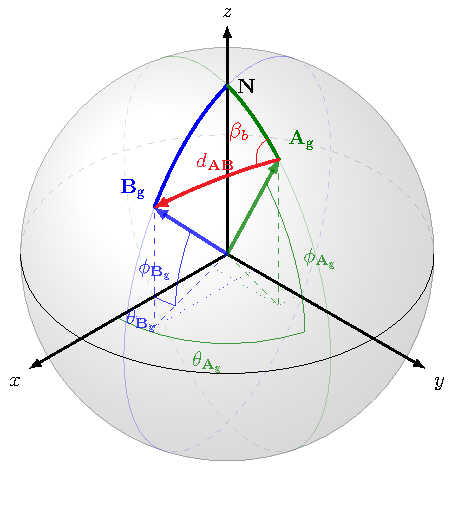
\includegraphics[width=0.95\textwidth]{../pictures/globo.pdf}
            \end{column}
            \begin{column}{0.45\textwidth}
                \begin{itemize}[<+->]
                    \item \textcolor{Green}{$A$} e \textcolor{Blue}{$B$} são coordenadas geográficas
                    \item \textcolor{Green}{$\theta_A$} e \textcolor{Blue}{$\theta_B$} são latitudes
                    \item \textcolor{Green}{$\phi_A$} e \textcolor{Blue}{$\phi_B$} são longitudes
                    \item Conhecendo essas informações, é possível determinar o ângulo \textcolor{Red}{$\beta$} relativo entre as duas coordenadas
                    \item Também é possível determinar sua distância
                \end{itemize}
            \end{column}
        \end{columns}
    \end{frame}

    \begin{frame}{Cálculo de Bearing}
        % \begin{multicols}{2}
            \begin{equation*}
                \Delta_\phi = \textcolor{Blue}{\phi_B} - \textcolor{Green}{\phi_A}
            \end{equation*}
            \begin{equation*}
                \Delta_\theta = \textcolor{Blue}{\theta_B} - \textcolor{Green}{\theta_A}
            \end{equation*}
            \begin{equation*}
                X = \cos\left(\textcolor{Blue}{\theta_B}\right)\cdot \sin\left(\Delta_\phi\right)
            \end{equation*}
            \begin{equation*}
                Y = \cos\left(\textcolor{Green}{\theta_A}\right)\cdot\sin\left(\textcolor{Blue}{\theta_B}\right) - \sin\left(\textcolor{Green}{\theta_A}\right) \cdot \cos\left(\textcolor{Green}{\theta_B}\right) \cdot \cos\left(\Delta_\phi\right)
            \end{equation*}
            \begin{equation*}
                Z = \sin^2\left(\frac{\Delta_\theta}{2}\right) + \cos\left(\textcolor{Blue}{\theta_B}\right) \cdot \cos\left(\textcolor{Green}{\theta_A}\right) \cdot \sin^2\left(\frac{\Delta_\phi}{2}\right)
            \end{equation*}
            \begin{equation*}
                \textcolor{Red}{\beta_b} = \arctan\left(\frac{X}{Y}\right)
            \end{equation*}
            \begin{equation*}
                d_{AB} = R_\text{Terra} \cdot 2 \cdot \arctan\left(\frac{\sqrt{Z}}{\sqrt{1-Z}}\right)
            \end{equation*}
        % \end{multicols}
    \end{frame}

